\subsubsection{System implementation}
The system is written in C\# using Microsoft Visual Studio 10. Since OpenCV\cite{opencv} is not compatible with C\# natively we use Emgu\cite{emgu} which is a wrapper for OpenCV to use in C\#. 

The design of the system has been done using UML diagrams. UML makes it easier knowing which parts communicated with other parts, their included methods and properties. The UML diagram for the PoolTracker can be seen in \ref{fig:uml}.

\begin{figure}[H]
\begin{center}
\leavevmode
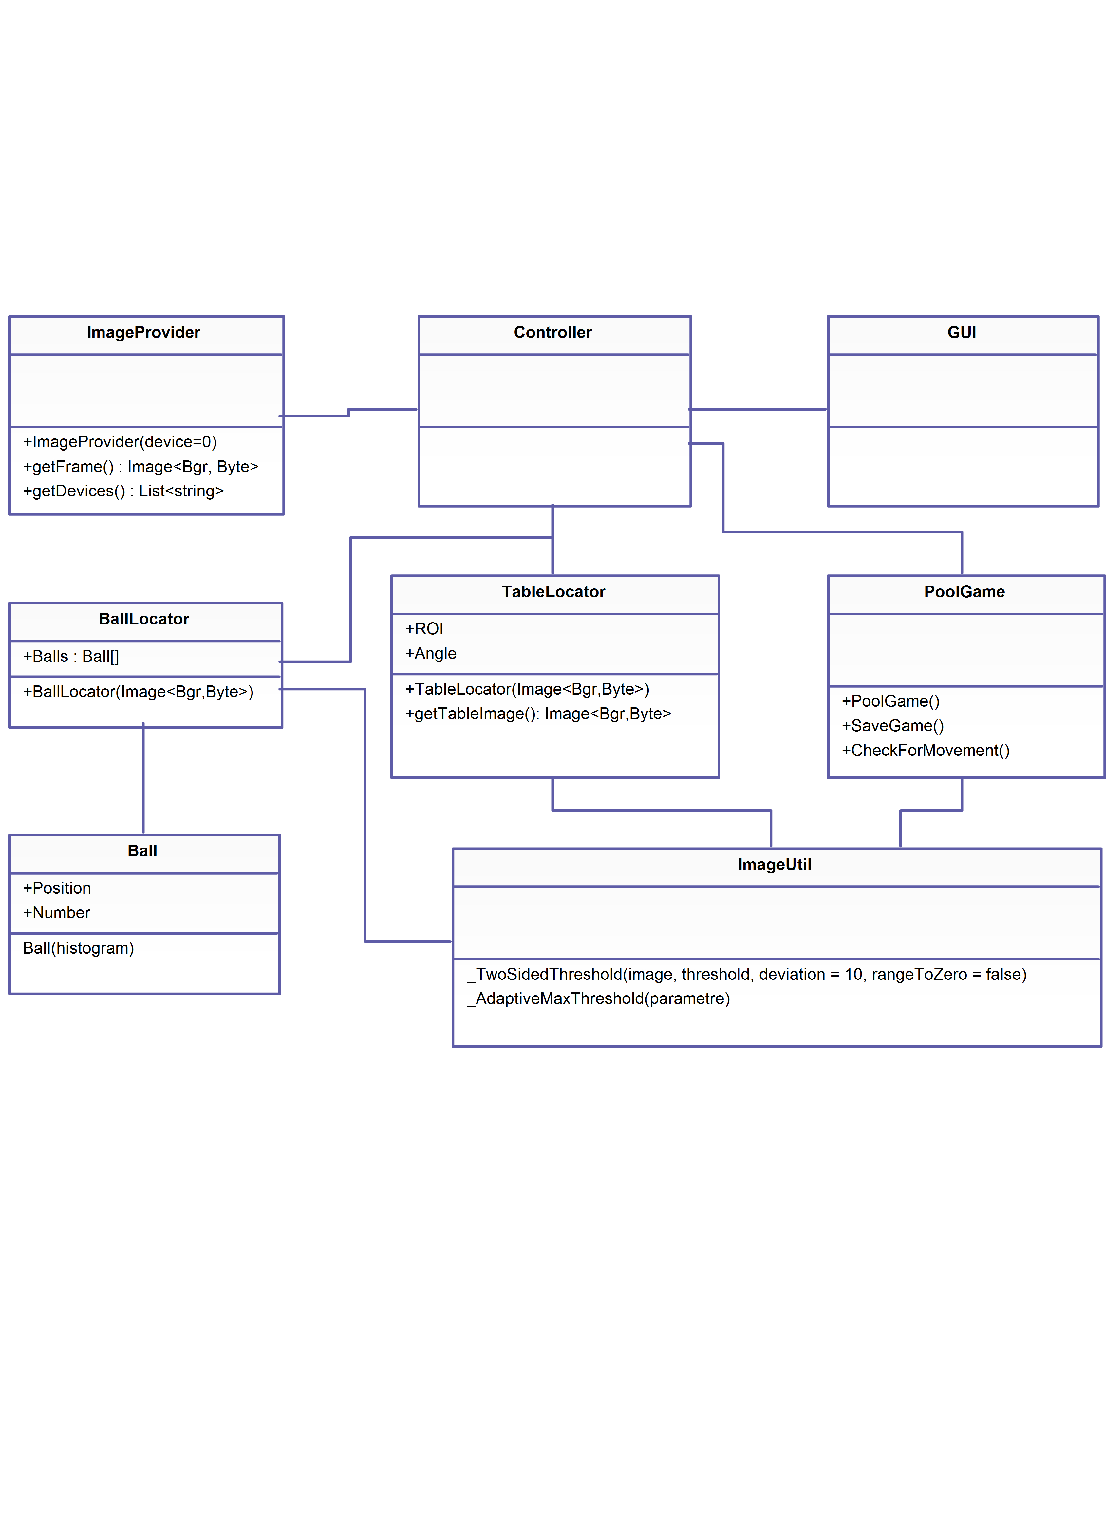
\includegraphics[width=0.8\textwidth]{images/UML}
\end{center}
\caption{UML diagram of PoolTracker.}
\label{fig:uml}
\end{figure}

\subsubsection{Calibration flow}
The calibration have to be done every time the camera changes position or when the system is installed for the first time. The calibration is done to locate table and to train the system with the colors of the balls. The calibration flowchart can be seen in \ref{fig:calib_flowchart}.\\

Table location is explained in \ref{sec:table-locate}.\\

\fixme{Train colors of balls? + insert flowchart}



\subsubsection{Program run flow}
The goal is to record a game of pool between every shots. To do this automatic, the program will have to know when a shot has been made and when to stop recording. The program flowchart can be seen in \ref{fig:program_flowchart}.\\

\begin{figure}[H]
\begin{center}
\leavevmode
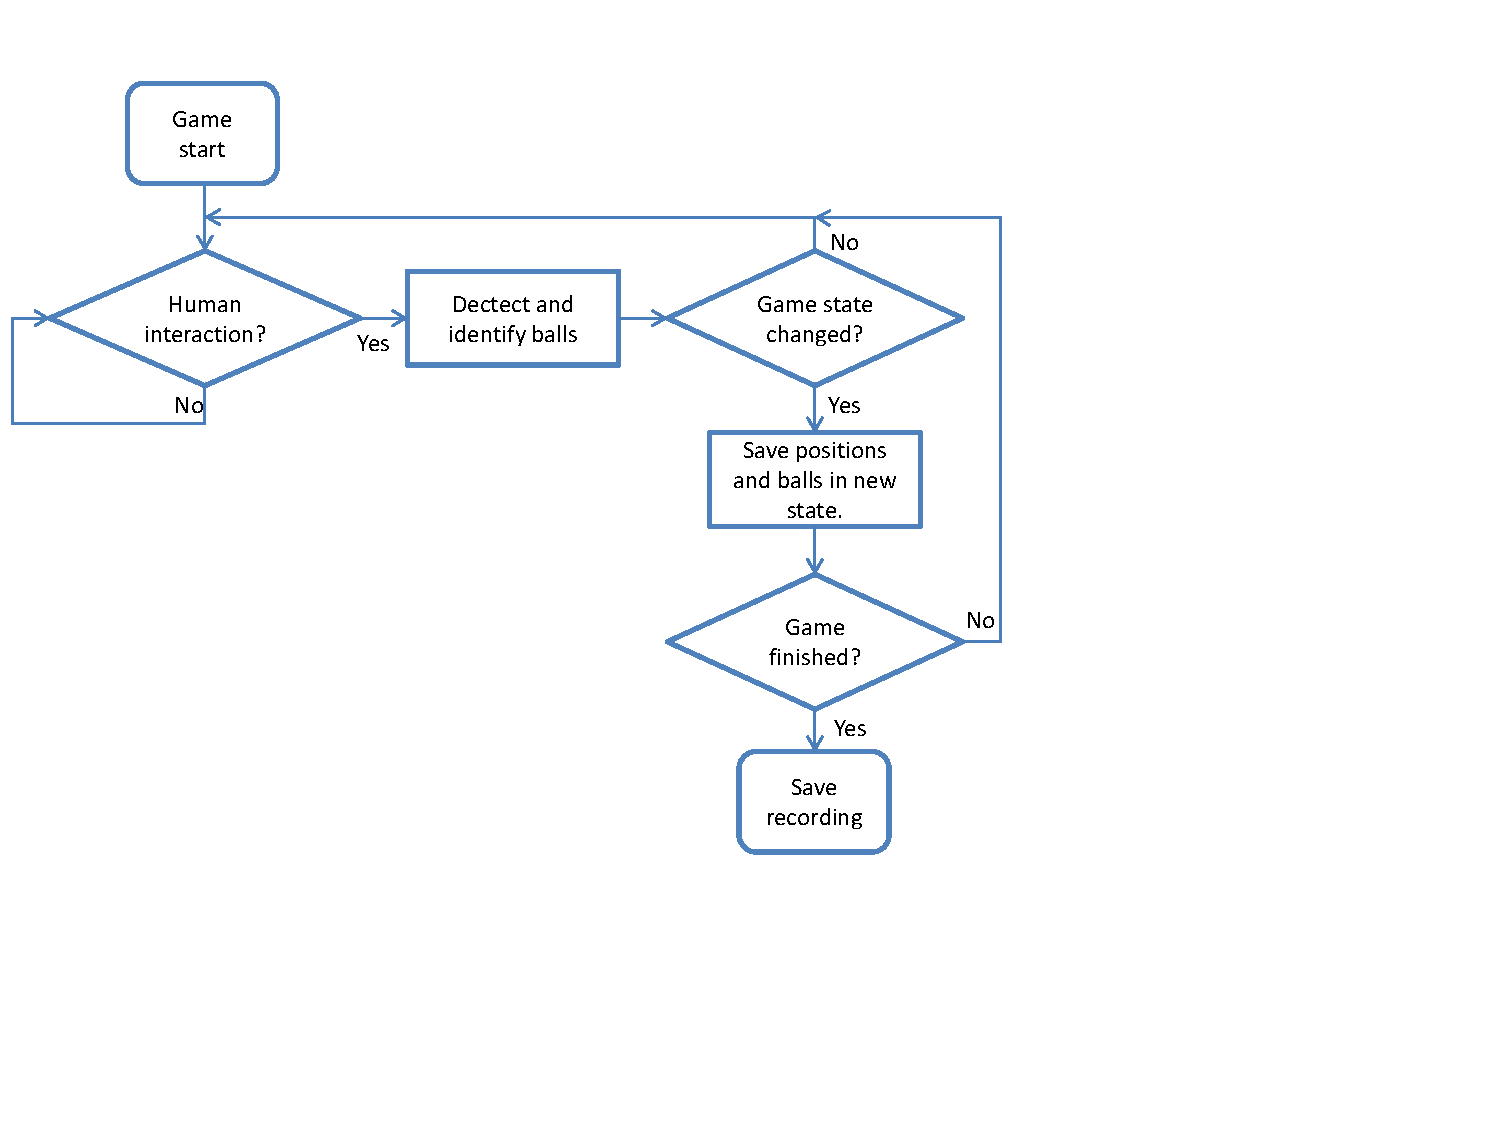
\includegraphics[width=0.8\textwidth]{images/program_flowchart}
\end{center}
\caption{Flowchart of the PoolTracker program while running.}
\label{fig:program_flowchart}
\end{figure}

The game will start when the user decides to do so. The detection of occlusions will be explained in \ref{sec:shotdetection}. The movement of balls will be detected in\ref{sec:shotdetection} based on the balls positions which will be found in \ref{sec:balls-locate}.